\chapter{Administration}
\label{administration}

\section{Hinzufügen von Fehler-Datenquellen}
\label{additional-error-source}
Die Applikation benutzt die View \inlinecode{kort.all\_errors} als Schnittstelle zu allen Fehlerdaten.
Wenn neue Fehlerquellen an das System angeschlossen werden sollen, dann muss entsprechend diese View angepasst werden.
Die jetzige View ist auf die Fehlerquelle Keepright (siehe Kapitel \ref{datenquellen-keepright}) angepasst.

Es werden einige Anforderungen an eine neue Fehlerquelle gestellt:
\begin{itemize}
\item Ein Fehler muss sich konkret auf ein OpenStreetMap-Objekt beziehen (Node, Way oder Relation)
\item Für die Darstellung auf der Karte muss ein einzelne Koordinate angegeben werden können (keine Flächen oder Wege)
\item Zu einem Fehler gibt es eine aussagekräftige Fehlermeldung
\end{itemize}

Die Fehler einer neuen Quelle müssen auf die bestehenden Fehlertypen gemappt werden.
Falls dies nicht geht oder es sich um neue Arten von Fehlern handelt, so müssen zusätzliche Fehlertypen eingeführt werden (siehe unten).

\section{Hinzufügen von Fehlertypen}
\label{additional-error-type}
Um neue Fehlertypen hinzuzufügen gibt es sowohl technische wie auch fachliche Anpassungen vorzunehmen.
Wichtig ist dabei den Endbenutzer nicht aus den Augen zu verlieren.
Alle aufgeführten Fehler sollten sich mit wenigen Eingaben lösen lassen.
Die bisher implementierten Fehlertypen benötigen alle nur eine einzige Eingabe.
Für neue Typen ist zu prüfen ob diese sich bereits mit den bestehenden Views abbilden lassen (siehe Kapitel \ref{view-types}).
Ist dies nicht der Fall, so muss eine neue View erstellt werden.

\subsection{Fehlertypen}
In der App sind bereits folgende Fehlertypen implementiert:

\begin{itemize}
\item Autobahn ohne Bezeichner
\item Kultstätte/Kirche ohne Religion
\item Objekt ohne Namen
\item Beziehung ohne Typ
\item Fehlendes Tempolimit
\item Sprache des Namens unbekannt
\item Typ des Wegs unbekannt
\item Strasse ohne Namen
\end{itemize}

Diese Typen sind in der Tabelle \inlinecode{kort.error\_type} definiert.
Im Feld \inlinecode{type} dieser Tabelle befindet sich die eindeutige Identifikation eines Typs.
Diese wird beispielsweise für die Anzeige eines passenden Marker-Icons (für die Karte) und der Verbindung zu einem passenden View-Typ (siehe Abschnitt \ref{view_types}) verwendet.

% IMAGE keepright.error_type
\begin{figure}[H]
	\centering
	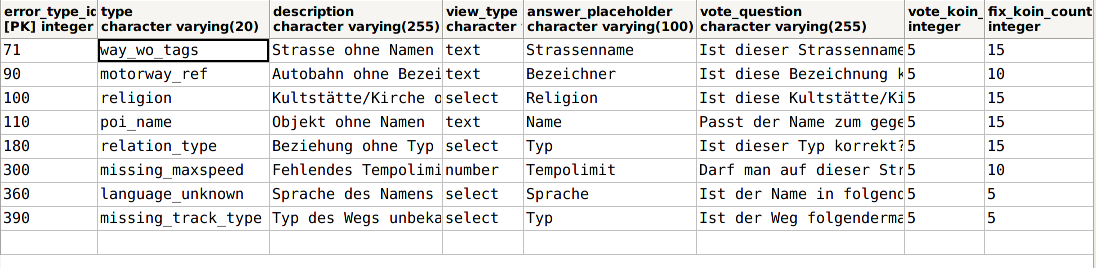
\includegraphics[width=\textwidth]{images/implementation/backend/table-error-type}
	\caption{Die Tabelle \inlinecode{kort.error\_type}}
\end{figure}

\subsubsection{Erstellen eines neuen Fehlertyps}
\label{create-new-error-type}
Ein neuer Fehlertyp muss in der Tabelle \inlinecode{kort.error\_type} hinzugefügt werden.
Sobald Fehler als \inlinecode{type} den neuen Typ eingetragen haben, wird dieser auch angezeigt.
Jeder Fehlertyp hat ein zugehörige Marker-Icon welches beispielsweise auf der Karte angezeigt wird.
Die Bilddatei hat den gleichen Namen wie das Attribut \inlinecode{type} und befindet sich im Ordner \inlinecode{/resources/images/marker\_icons}.

\subsection{View-Typen}
\label{view-types}
All diese Typen werden dann wiederum einem spezifischen View-Typen zugeordnet.
Dieser bestimmt, wie das Formular zum Lösen des Fehlers in der Benutzeroberfläche aussieht.

In Tabelle \ref{kort-view-types-table} sind die bereits vorhandenen View-Typen beschrieben.

\begin{table}[H]
\centering
\begin{tabular}{|p{0.15\twocelltabwidth}|p{0.85\twocelltabwidth}|}
\hline
\textbf{Typ} & \textbf{Beschreibung} \\
\hline
\inlinecode{text} & Rendert ein Text-Eingabefeld \\
\hline
\inlinecode{number} & Rendert ein Zahl-Eingabefeld \\
\hline
\inlinecode{select} & Rendert eine Select-Box mit vorgefüllten Werten aus der Datenbank \\
\hline
\end{tabular}
\caption{kort: View-Typen}
\label{kort-view-types-table}
\end{table}

Wird als View-Typ \emph{select} gewählt, müssen in der Tabelle \inlinecode{kort.answer} noch die möglichen Antworten eingetragen werden.
Darin kann der eigentliche Wert des OpenStreetMap-Tags und eine passende Bezeichnung hinterlegt werden.
Als \inlinecode{type} muss der jeweilige Typen-Bezeichner gewählt werden.

\subsubsection{Erstellen eines neuen View-Typen}
Um einen neuen View-Typen zu definieren muss wie in Code-Ausschnitt \ref{kort-add_view_type} beschrieben die Unterscheidung in der Klasse \inlinecode{Kort.view.bugmap.fix.Form} um den neuen Typen ergänzt werden.

\lstset{language=JavaScript}
\begin{lstlisting}[float, caption=Hinzufügen eines View-Typen in der Klasse Kort.view.bugmap.fix.Form, label=kort-add_view_type]
createFixField: function(bug) {
	[...]
	
	if(bug.get('view_type') === '<Neuer View-Typ>') {
		fixField = Ext.create('<Neue View-Klasse>', fieldConfig);
	} else {
		...
	}
	
	[...]
}
\end{lstlisting}

\section{Hinzufügen von Auszeichnungen}
\label{kort-additional-badges}
Die bereits vorhandenen Auszeichnungen sind in Tabelle \ref{kort-badges} beschrieben. Um weitere Auszeichnungen hinzuzufügen, muss folgendermassen vorgegangen werden:

\begin{enumerate}
\item Es muss ein neuer \gls{Badge} in der Tabelle \inlinecode{kort.badge} erstellt werden
\item Zusätzlich muss eine Regel für das Gewinnen des \gls{Badge}s in der Methode \inlinecode{RewardHandler::updateBadges()}\footnote{\url{http://kort.herokuapp.com/docs/Kort-backend/classes/Webservice.RewardHandler.html\#method_updateBadges}} hinzugefügt werden.
\item Für das Frontend muss ein Bild erstellt werden, welches dem Namen (Tabellenattribut \inlinecode{kort.badge.name}) des \gls{Badge}s entspricht. Dieses Bild muss in folgendem Pfad gespeichert werden \inlinecode{/resources/images/badges/<badgename>.png}.
\end{enumerate}

Sind alle Punkte abgearbeitet ist der \gls{Badge} im Frontend ersichtlich und kann von den Benutzern gewonnen werden.

\section{Hinzufügen von OAuth Anbietern}
\label{kort-additional-oauth-provider}
Derzeit ist der Login über Googles \gls{OAuth}-Dienst möglich, um zukünftig weitere Login-Dienste anbieten zu können müssen einige Schritte beachtet werden.
Der Dienst muss folgende Anforderungen erfüllen:
\begin{itemize}
\item Unterstützung für OAuth 1.0 oder 2.0
\item Offline-Zugang, d.h. es müssen Aktionen ohne den Benutzer möglich sein
\item Ein längerfristig gültiges Token, welches als \emph{Refresh Token} bezeichnet wird
\item Der Dienst muss eine Registrierung der Applikation ermöglichen
\end{itemize}

Wenn ein Dienst diese Anforderung erfüllt, muss die Applikation registriert werden.
Die Angaben für Google sind dabei im Kapitel \ref{oauth} vermerkt.

Im Backend kann eine entsprechende Subklasse von \inlinecode{AbstractOAuthCallback}\footnote{\url{http://kort.herokuapp.com/docs/Kort-backend/classes/OAuth.AbstractOAuthCallback.html}} erstellt werden. 
Eine so erstellte OAuthCallback-Klasse nimmt dann einen Callback des entsprechenden Anbieters entgegen und authentifiziert den Benutzer.
Das zugehörige Callback-Script wird im Order \inlinecode{/server/oauth2callback} gespeichert.

Schlussendlich muss das Frontend noch angepasst werden.
Dazu gehört, dass der neue Dienst in der Konfiguration (siehe Kapitel \ref{frontend-config}) eingetragen werden muss.
Um einen neuen Login-Button anzuzeigen muss dieser auch noch auf dem Login-Panel (\inlinecode{/app/view/overlay/login/Panel.js}) hinzugefügt werden.
Die zugehörige Logik befindet sich im Login-Controller (\inlinecode{/app/controller/Login.js}).
\begin{figure}[H]
	\centering
	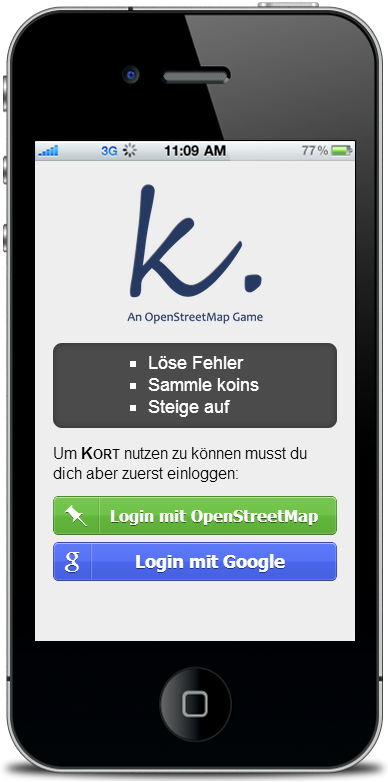
\includegraphics[scale=0.5]{images/screenshots/kort-screenshot-login}
	\caption{Login-Button des OAuth-Anbieters}
\end{figure}


\section{Reset der Applikation}
\label{kort-reset}
Um die Applikation zurückzusetzen kann die Stored Procedure \inlinecode{reset\_kort()} verwendet werden. 
Die Prozedur löscht alle laufenden Daten aus der Datenbank, so dass wieder der Ursprungszustand hergestellt ist:
\begin{itemize}
\item Die Punkte (\emph{\gls{koins}}) aller Benutzer werden auf 0 zurückgesetzt
\item Die \gls{Badge}s aller Benutzer werden entfernt
\item Alle Lösungsvorschläge von Benutzern werden entfernt
\item Alle Überprüfungen von Lösungsvorschlägen werden entfernt
\end{itemize}

Auf Aufruf der Prozedur sieht wiefolgt aus:
\begin{lstlisting}[float, caption=Aufruf von reset\_kort() um die Applikation zurückzusetzen, label=kort-reset-cmd]
select reset_kort();

 reset_kort 
------------
 t
(1 row)
\end{lstlisting}

Die Prozedur liefert \inlinecode{true} wenn alles geklappt hat, ansonsten \inlinecode{false}.

\section{Frontend Kofiguration}
\label{frontend-config}
Die Konfiguration des Frontends befindet sich in der Datei \inlinecode{/app/util/Config.js}.
Darin sind alle Parameter definiert, welche die Applikation für den Betrieb benötigt.

In der \textsc{Kort}-Dokumentaton sind alle Parameter detailliert beschrieben: \url{http://kort.herokuapp.com/docs/Kort/#!/api/Kort.util.Config}